%!TEX ROOT=main.tex
\chapter{Implementace}
V této kapitole je popsaná realizace systému CarDi a naměřené hodnoty pneumatického systému.

\section{Deska plošného spoje}
Na desce plošného spoje (DPS) sídlí všechny elektrické komponenty systému. DPS a schéma je navržena v otevřeném freeware KiCad EDA.
\begin{figure}[H]
    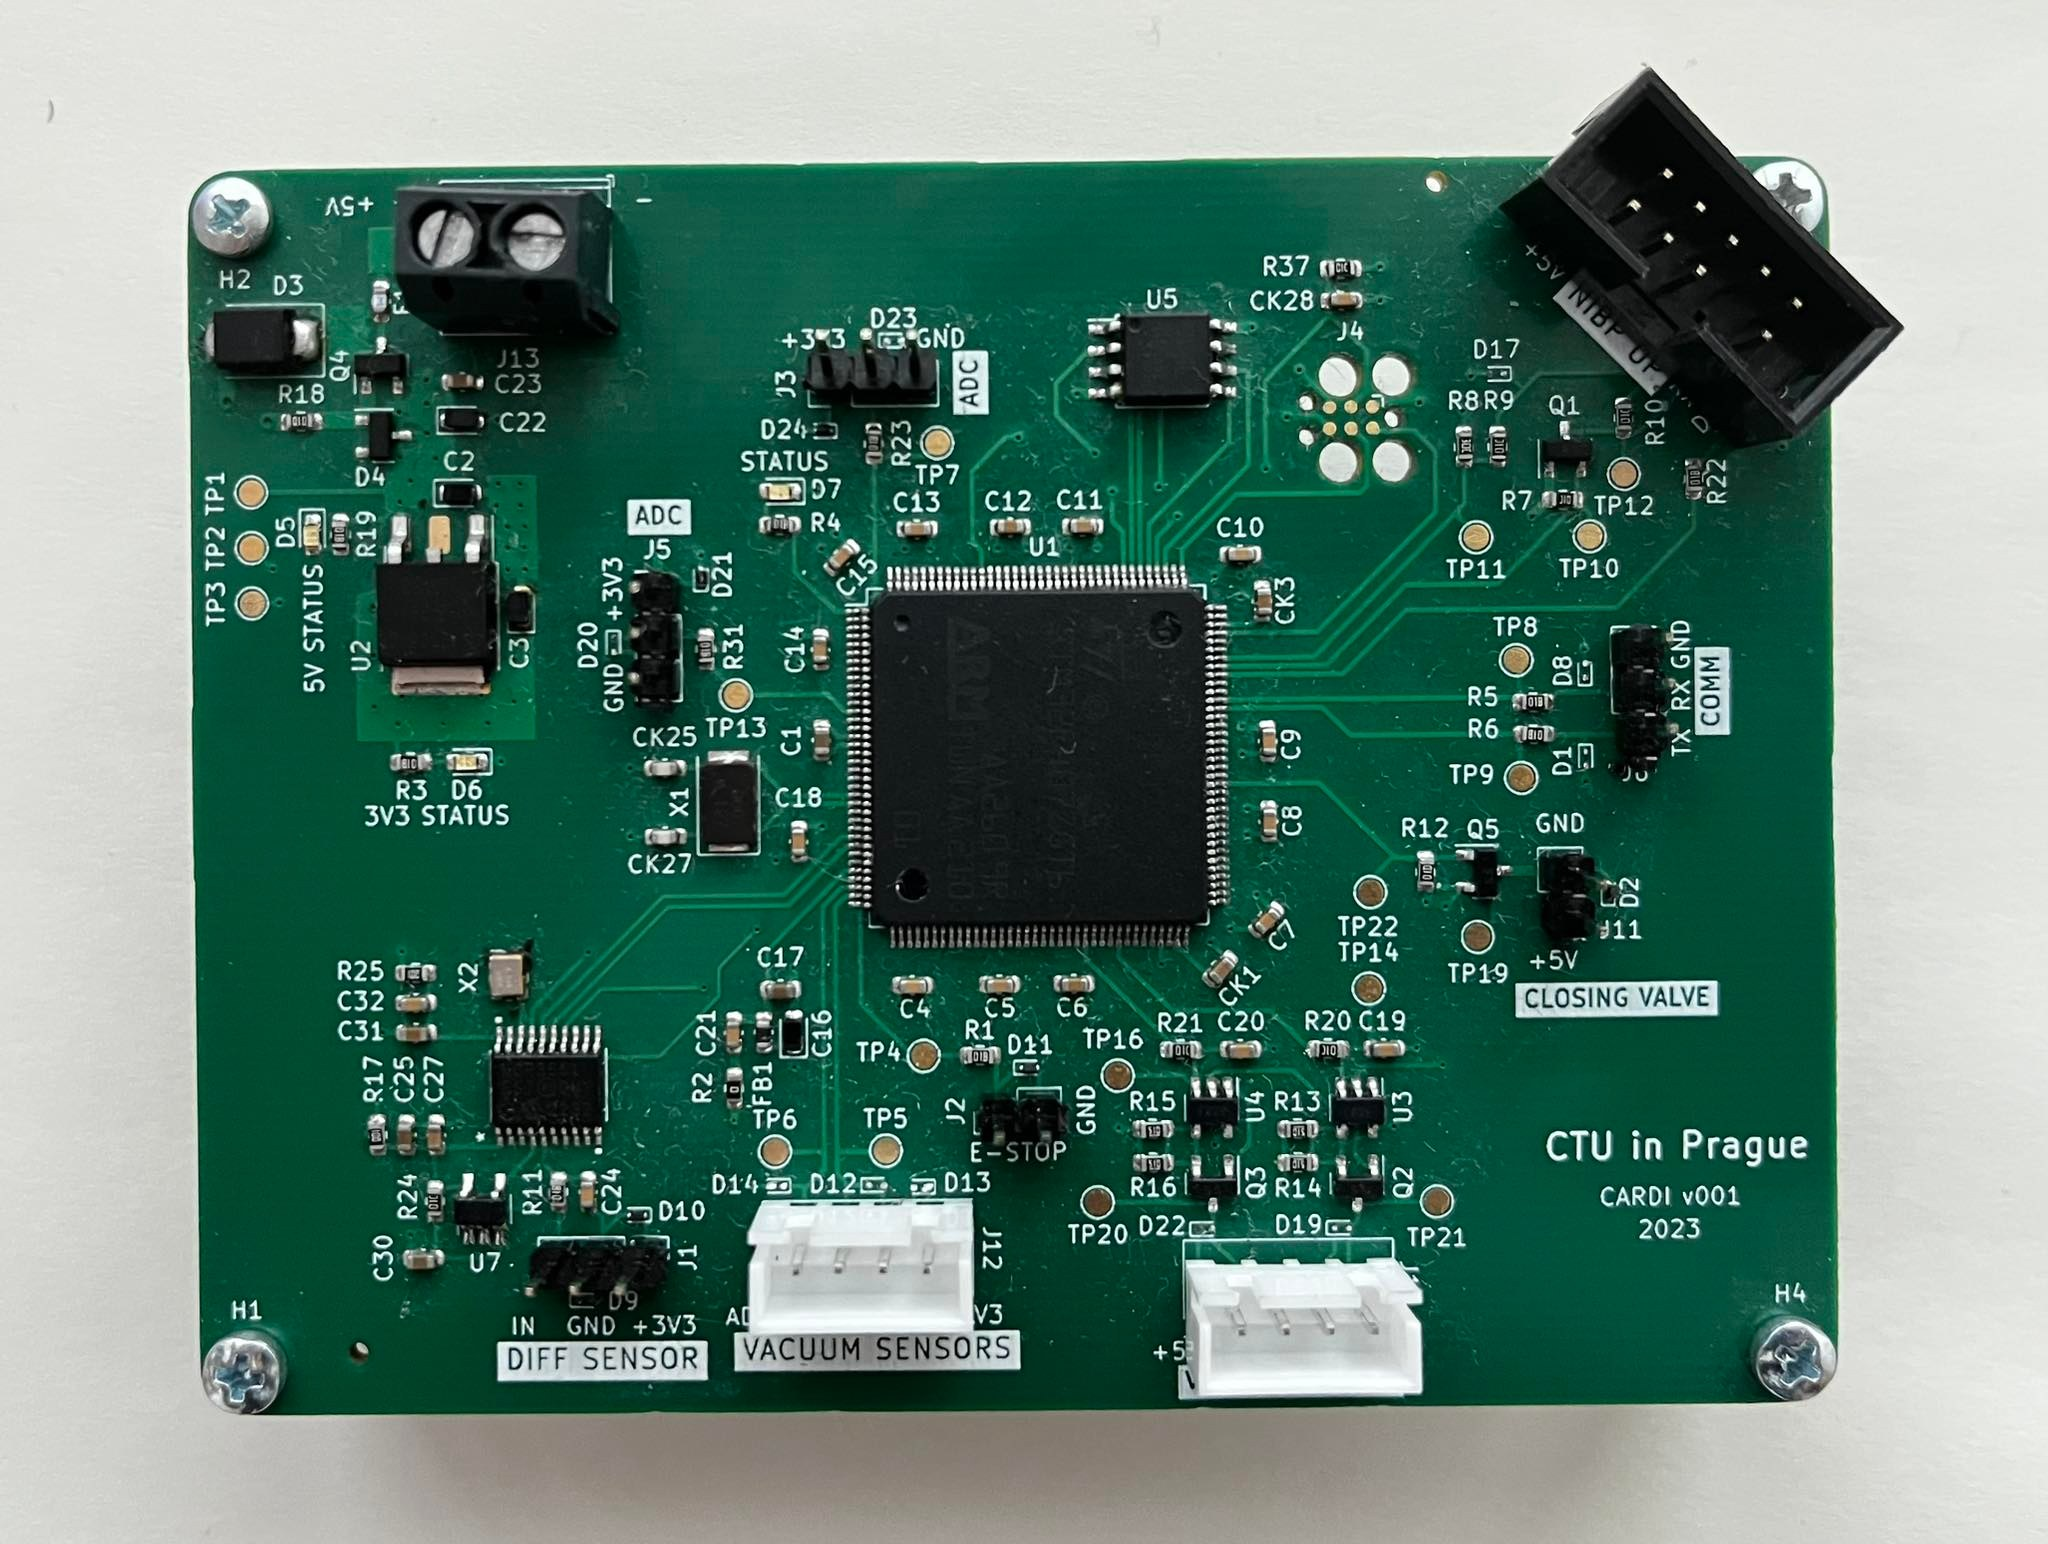
\includegraphics[width=1\linewidth]{pictures/pcb_full.jpg}
    \caption{Realizovaná deska plošného spoje.}
    \label{fig:pcb_full}
\end{figure}

DPS je čtyřvsrtvá deska s dvěma signálovými vrstvy a dvěma silovýma vrstvama. Kde první(horní) vrstva je signálová a nachází se na ní veškeré elektronické komponenty. Druhá je společná zem, třetí je napájencí 3.3 V a poslední spodní vrtva je také signálová.
Základní materiál je FR-4 a povrchová úprava je ENIG(Electroless nickel immersion gold).
\par
DPS je vyrobena a z části osazena firmou JLCPCB.
\begin{figure}[H]
    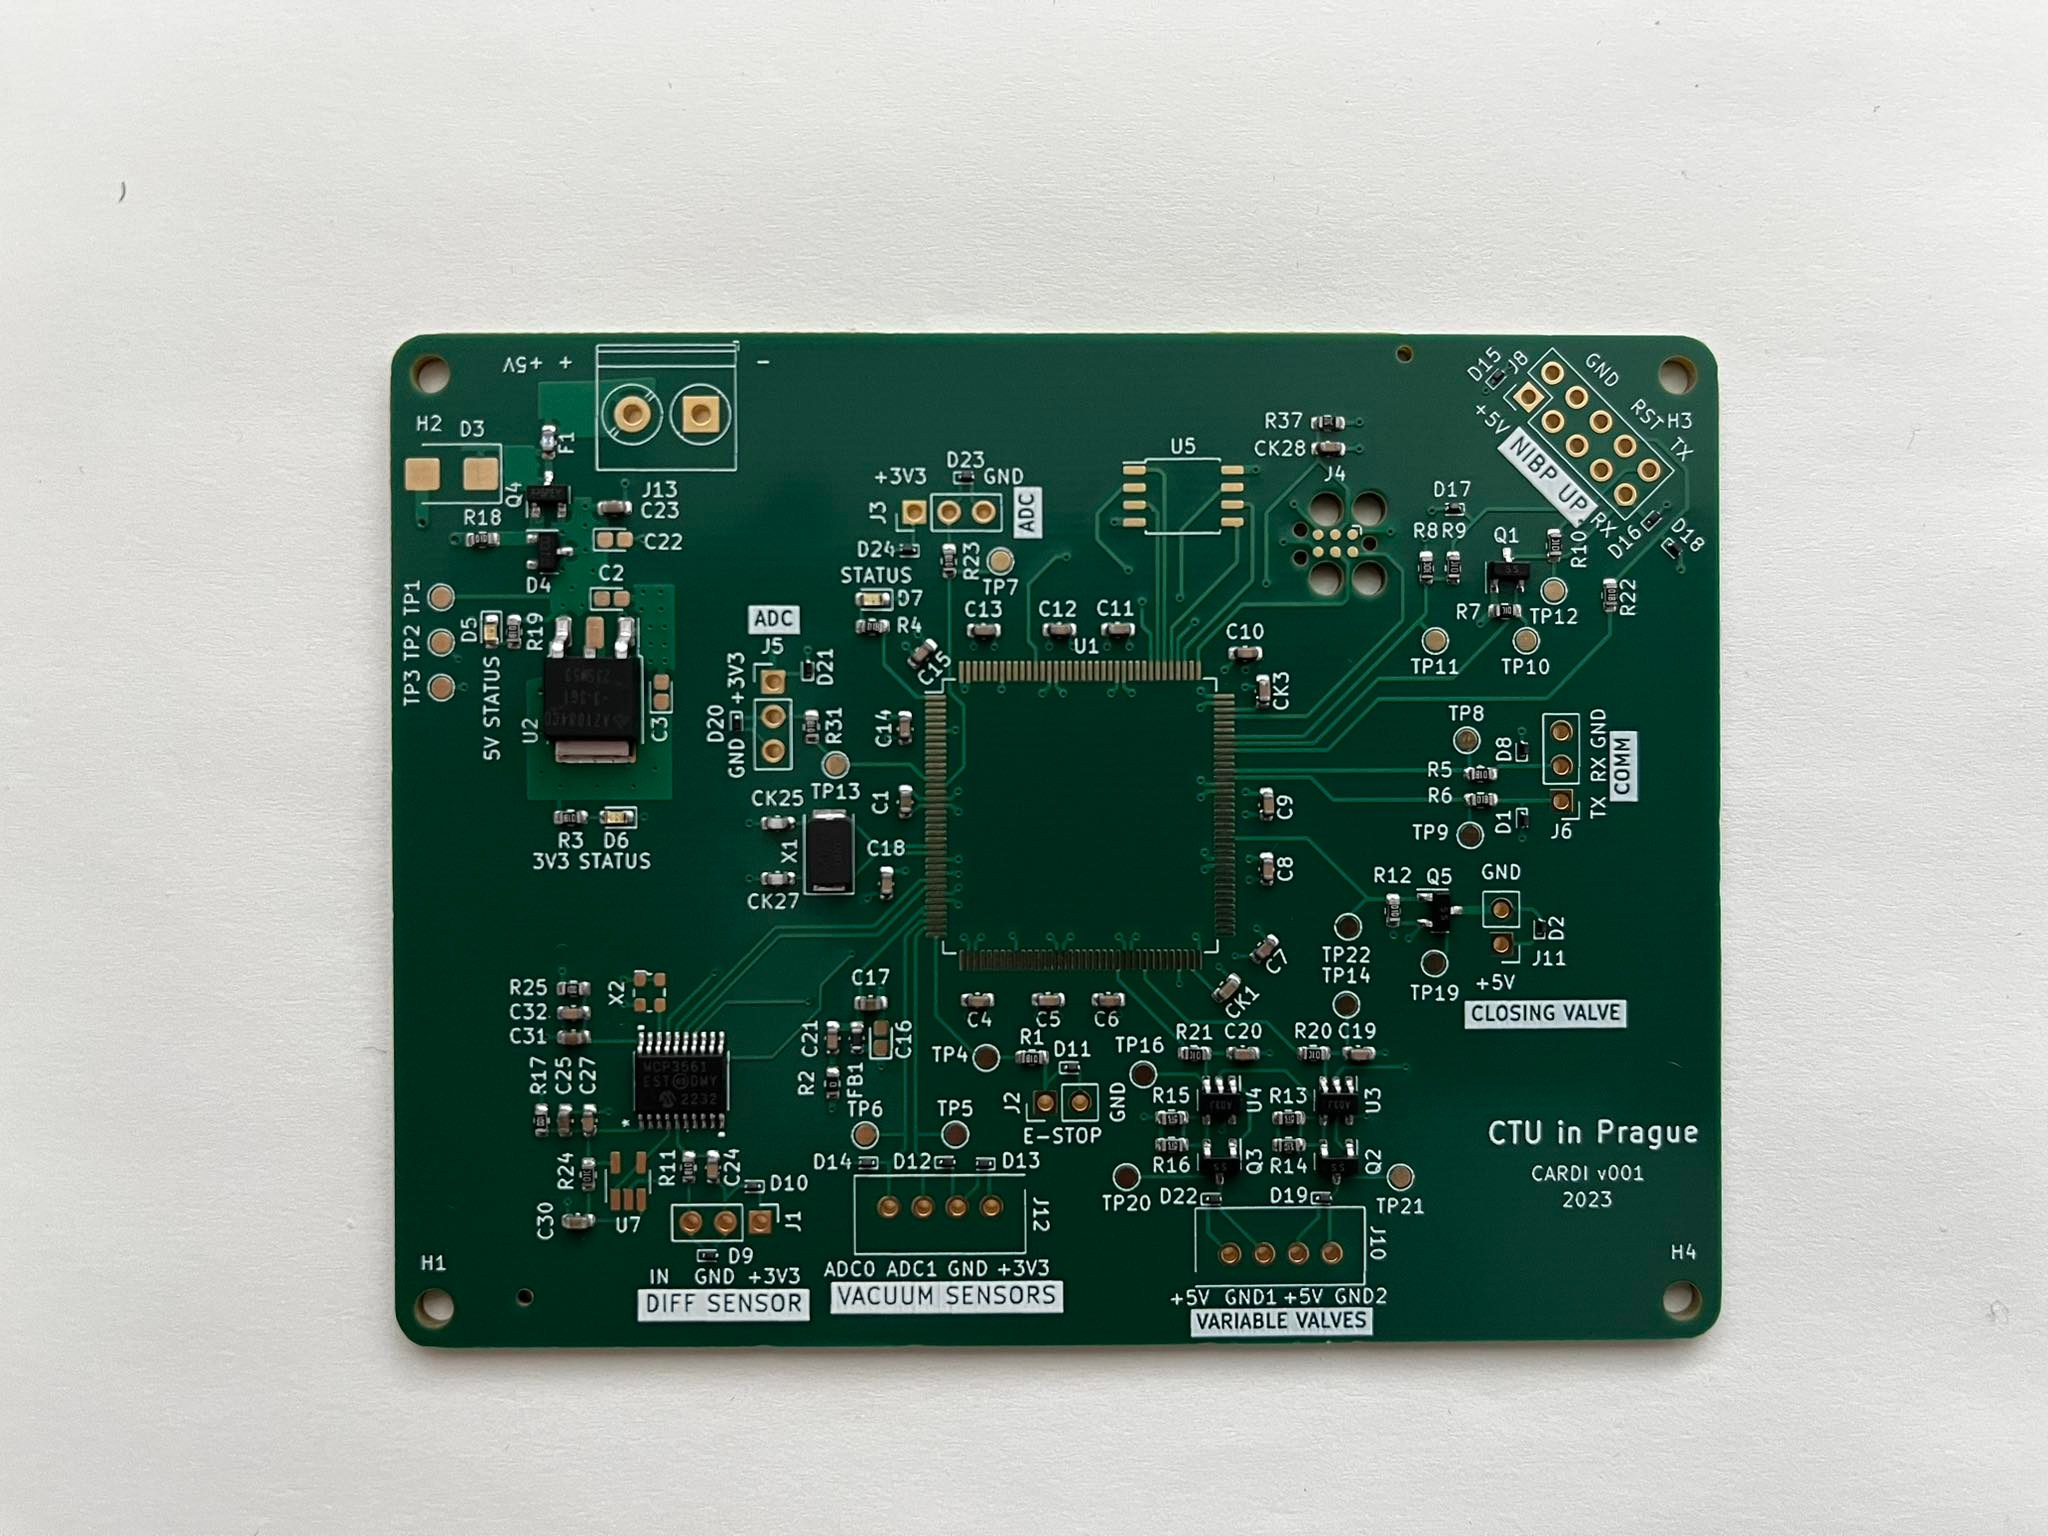
\includegraphics[width=1\linewidth]{pictures/pcb_from_production.jpg}
    \caption{Deska plošného spoje z výroby.}
    \label{fig:pcb_production}
\end{figure}
\begin{figure}[H]
    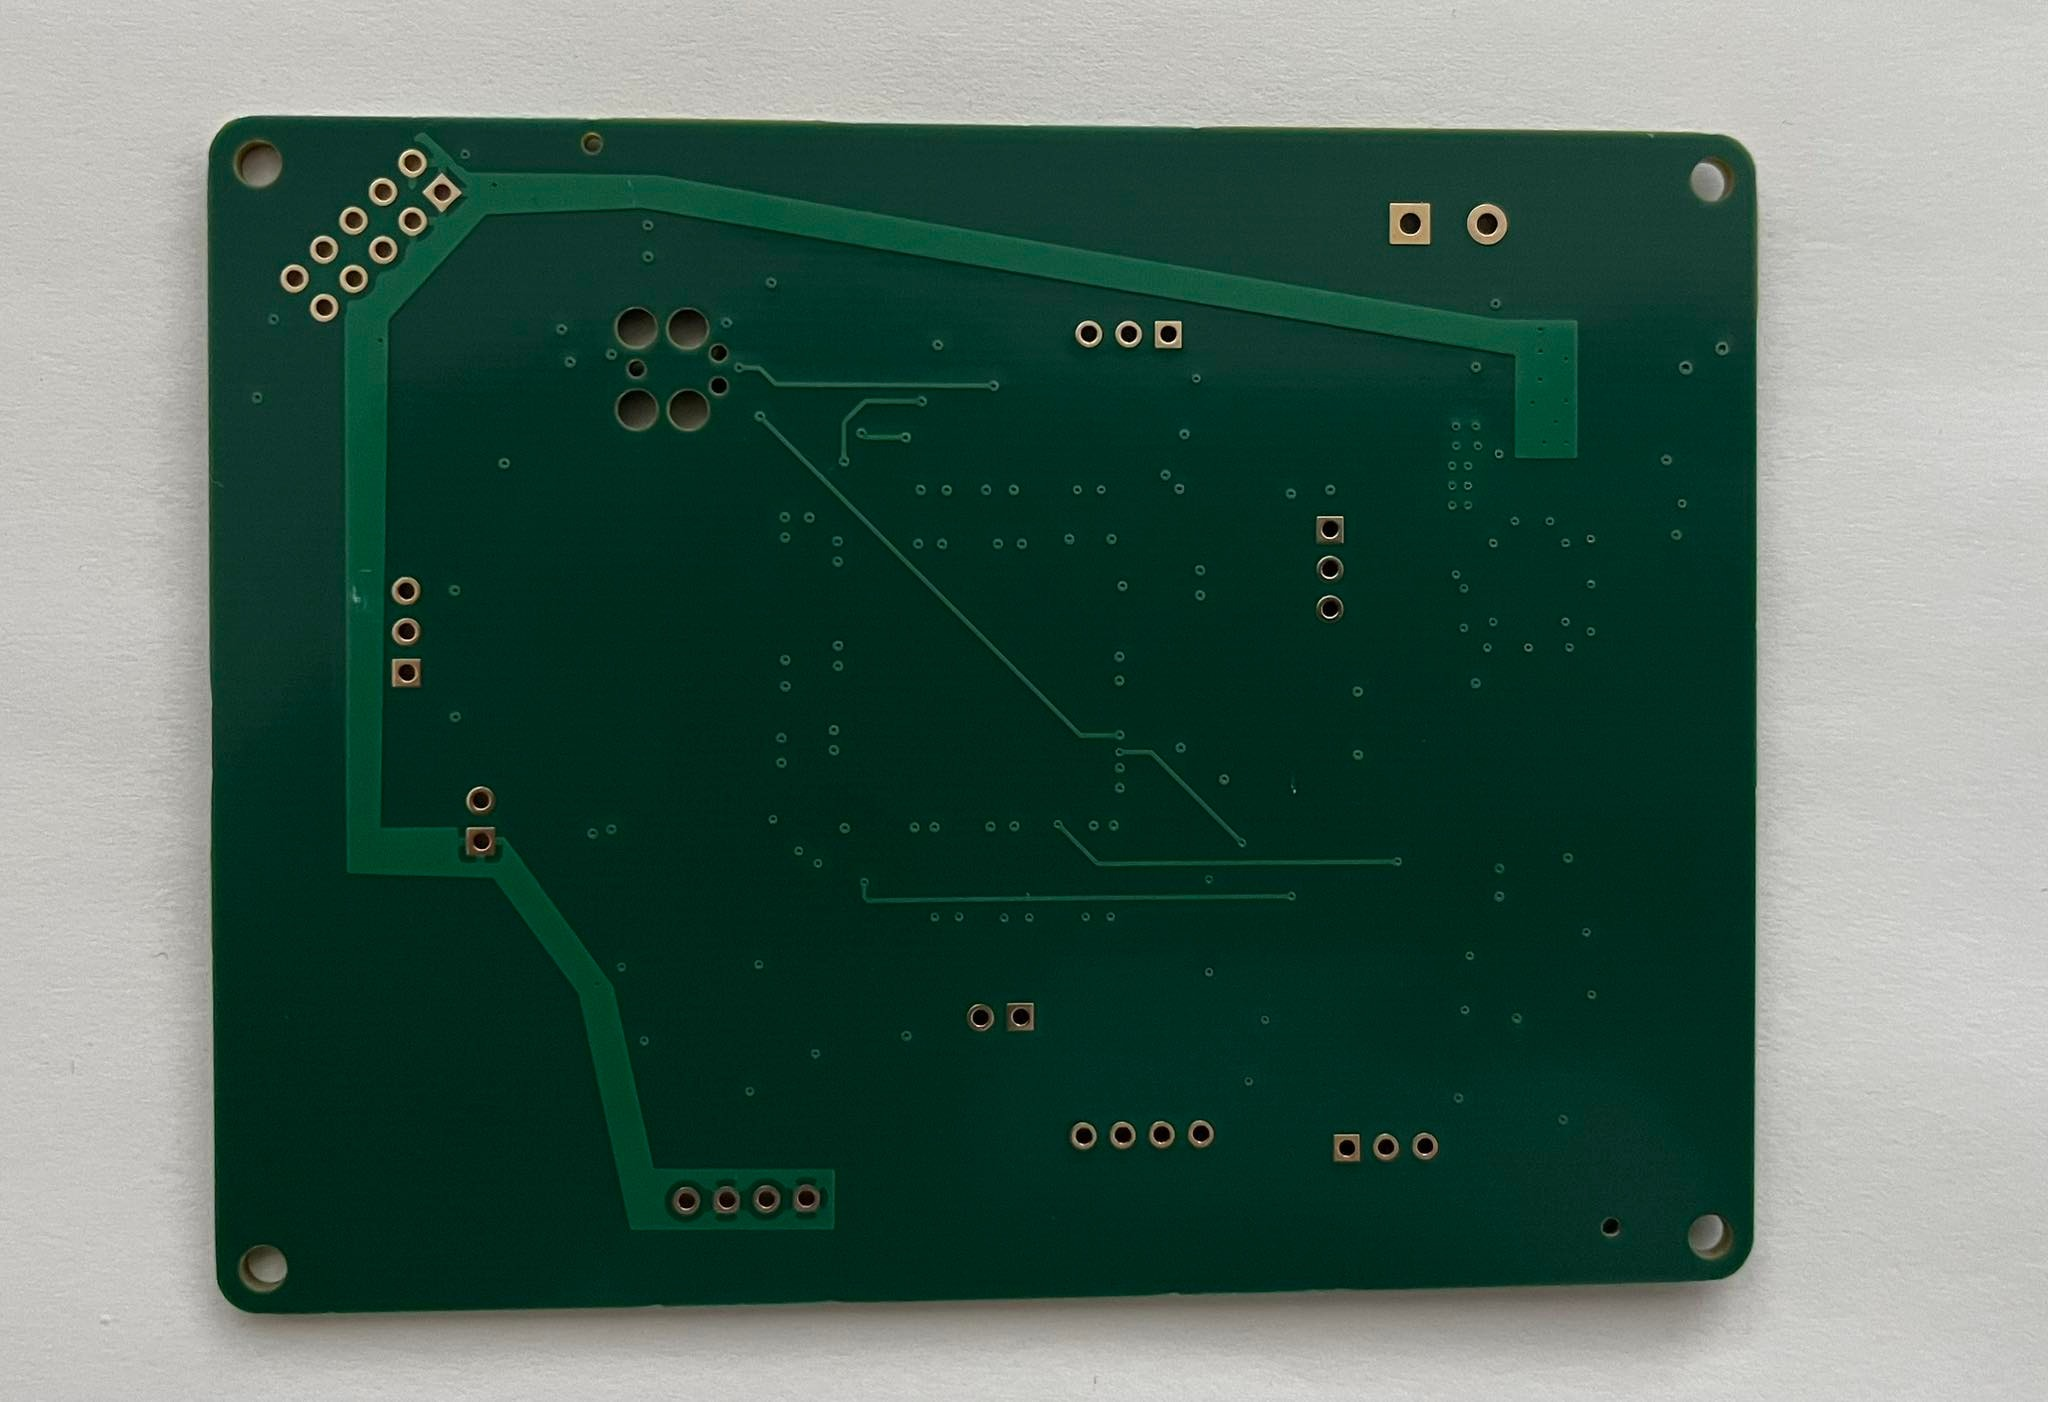
\includegraphics[width=1\linewidth]{pictures/pcb_production_bottom.jpg}
    \caption{Deska plošného spoje z výroby. Spodní vrstva.}
    \label{fig:pcb_production_bottom}
\end{figure}

Celkovká cena desky a potřebné materiály jsou:

\begin{table}[H]
    \label{tab:bom}
    \caption{Celkový počet součástek a výrobní cena }
    \begin{ctucolortab}
        \begin{tabular}{ccccccc}
            \toprule
            Typ                   & Název                  & Hodnota       & Počet & Cena     & Jednotky & \\ \midrule
            Kondenzátor           &                        & 100 nF        & 10    & 0.022    &          & \\
            Kondenzátor           &                        & 22 pF         & 2     & 0.0174   &          & \\
            Kondenzátor           &                        & 1 uF          & 4     & 0.018    &          & \\
            Kondenzátor           &                        & 2.2 uF        & 2     & 0.0096   &          & \\
            Kondenzátor           &                        & 4.7 uF        & 1     & 0.0091   &          & \\
            Kondenzátor           &                        & 10 uF         & 1     & 0.006    &          & \\
            Kondenzátor           &                        & 22 uF         & 3     & 0.015    &          & \\
            Resistor              &                        & 51 $\Omega$   & 4     & 0.5688   &          & \\
            Resistor              &                        & 10 $\Omega$   & 2     & 0.0032   &          & \\
            Resistor              &                        & 20 $k\Omega$  & 5     & 0.005    &          & \\
            Resistor              &                        & 10 $k\Omega$  & 7     & 0.0056   &          & \\
            Resistor              &                        & 0 $\Omega$    & 1     & 0.001    &          & \\
            Resistor              &                        & 1 $k\Omega$   & 10    & 0.005    &          & \\
            Resistor              &                        & 100 $k\Omega$ & 2     & 0.002    & €        & \\
            Dioda                 & BZX84C10VLT116         &               & 1     & 0.2264   &          & \\
            Dioda                 & D5V0F1U2S9-7           &               & 19    & 3.0837   &          & \\
            Dioda                 & SM6T6V8AY              &               & 1     & 0.1372   &          & \\
            Dioda                 & LED Green              &               & 3     & 0.0717   &          & \\
            IO                    & AZ1084CD-3.3TRG1       &               & 1     & 0.2395   &          & \\
            IO                    & MCP3561-E/ST           &               & 1     & 5.5941   &          & \\
            IO                    & MCP6001RT-I/OT         &               & 2     & 0.486    &          & \\
            IO                    & MCP6V91T-E/OT          &               & 1     & 1.81     &          & \\
            IO                    & MX25R3235FM2IL0        &               & 1     & 0.88     &          & \\
            IO                    & STM32F407ZGT6          &               & 1     & 1.02     &          & \\
            MOSFET                & TPM9305PS3-1           &               & 1     & 0.0958   &          & \\
            MOSFET                & BSS138                 &               & 4     & 0.09     &          & \\
            Ferritový korálek     & MPZ1608S102ATA00       &               & 1     & 0.0196   &          & \\
            Oscilátor             & ABM3-8.000MHZ-D2Y-T    & 8 MHz         & 1     & 0.5783   &          & \\
            Oscilátor             & ECS-2520MVLC-049       & 4.9152 MHz    & 1     & 1.23     &          & \\
            Pojistka              & F0603FF4000V032TM      & 4 A           & 1     & 0.0762   &          & \\
            \bottomrule
            $\Sigma$              &                        &               & 94    & 16.3262  & €        & \\
            \bottomrule
            Služba                & Výroba PCB od JLCPCB   &               & 1     & 5        & €        & \\
            Služba                & Osazení PCB            &               & 1     & 16       & €        & \\
            \bottomrule
            $\Sigma$              &                        &               & 2     & 21       & €        & \\
            \bottomrule
            Programátor           & ST-LINK/V2-ISOL        &               & 1     & 76.99    & €        & \\
            Kabel na programování & Tag Connect TC2030 IDC &               & 1     & 40.37    & €        & \\
            \bottomrule
            $\Sigma$              &                        &               & 2     & 117.36   & €        & \\
            \bottomrule
            \bottomrule
            $\Sigma$              & Bez DPH                &               &       & 154.6862 & €        & \\
            \bottomrule
        \end{tabular}
    \end{ctucolortab}
\end{table}
\section{Pneumatická část}

Pneumatická čast systému je část ve které probíhá měření měření hemodynamických parametrů srdce pacienta. Je to jediná čast systému, která přichází v přímý kontakt s pacientem.
\begin{figure}[H]
    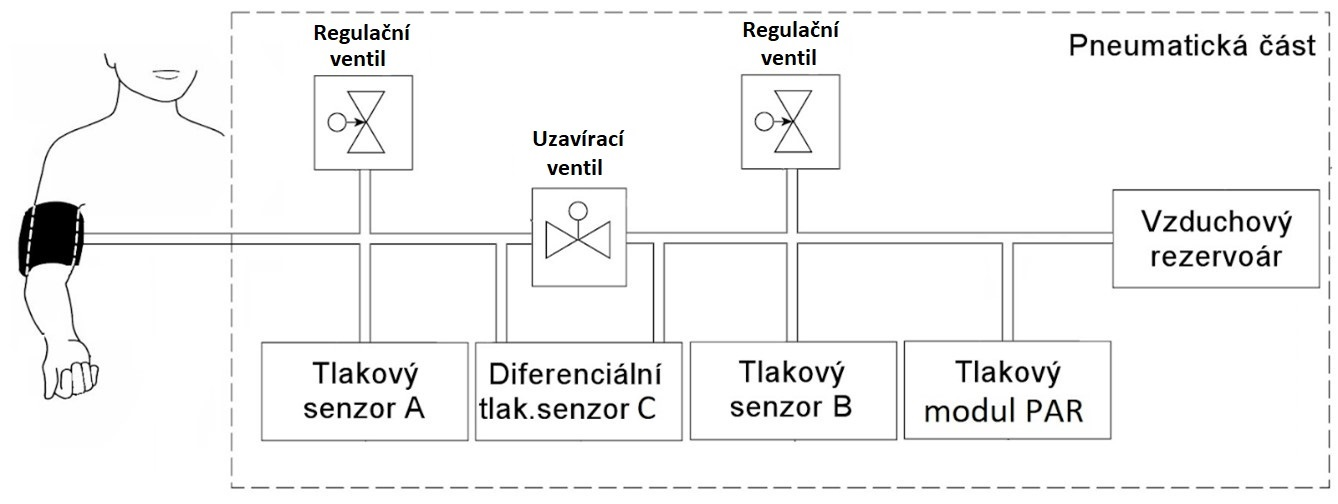
\includegraphics[width=1\linewidth]{pictures/blokove_schema_pneu.jpg}
    \caption{Blokové schéma pneumatického systému}
    \label{fig:pneu_block}
\end{figure}

\subsection{Měření těsnosti penumatické časti}
Pneumatická čast musí být co nejlépe těsná, aby po dobu terapie byl co nejmešní úbytek tlaku v systému.
\par
Test těsnosti probíhal pomocí přístroje FLUKE Biomedical BP pump 2, který natlakoval pneumatickou část na hodnotu 200 mmHg a následně sledoval úbytek tlaku v systému po dobu 60 s.
Měření bylo opakováno 10 krát po sobě.

\begin{table}[H]
    \label{tab:pressure_test_pneu}
    \caption{Test těstnosti pneumatického systému}
    \begin{ctucolortab}
        \begin{tabular}{ccc}
            \toprule
            Měření & Těsnost & Jednotky           \\ \midrule
            1      & 0.9     &                    \\
            2      & 0.8     &                    \\
            3      & 1.1     &                    \\
            4      & 1.0     &                    \\
            5      & 0.9     & $\frac{mmHg}{min}$ \\
            6      & 0.9     &                    \\
            7      & 1.1     &                    \\
            8      & 0.9     &                    \\
            9      & 0.8     &                    \\
            10     & 1.0     &                    \\
            \bottomrule
        \end{tabular}
    \end{ctucolortab}
\end{table}
Průměrný pokles tlaku v důsledku úniku vzduchu z pneumatického obvodu je $0.94 \ \frac{mmHg}{min}$ se směrodatnou odchylkou $0.10  \ \frac{mmHg}{min}$. Dle normy je maximální úbytek tlaku v systému $4 \ \frac{mmHg}{min}$.
\subsection{Zkreslení signálu pneumatickým systémem}
Přenosová funkce systému byla identifikována měřením impulzní odezvy systému. Systém byl natlakovám na průměrnou hodnotu suprasystolického tlaku 230 mmHg a poté
byl aplikován jednotkový impuls pomocí mechanického kyvadla.
\begin{figure}[H]
    \label{fig:mech_kyvadlo}
    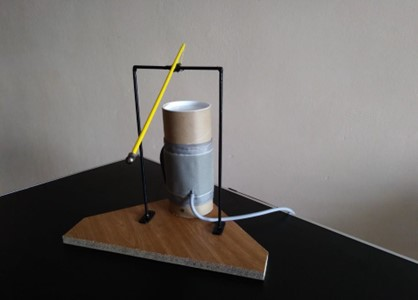
\includegraphics[width=1\textwidth]{pictures/mech_kyvadlo.jpg}
    \caption{Mechaniké kyvadlo pro vytvoření jednotkového impulsu na pneumatický systém.}
\end{figure}
\begin{figure}[H]
    \label{fig:pneu_impulse_response}
    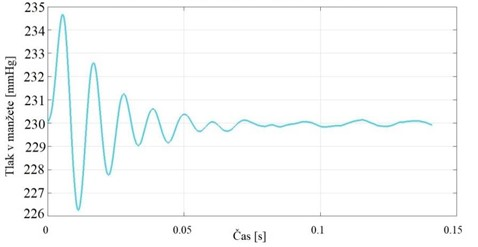
\includegraphics[width=1\textwidth]{pictures/pneu_impulse.jpg}
    \caption{Odezva pneumatického systému na jednotkový impuls.}
\end{figure}
Z naměřené hodnoty impulzní odezvy byly vypočteny parametry vlastní frekvence $f_0 \ [Hz]$ a poměrného útlumu $\xi \ [-]$. Pomocí těchto parametrů, za předpokladu, že se jedná o dynamický systém druhého řádu, bylo možné vypočítat přenosovou funkci systému.
\begin{figure}[H]
    \caption{Odezva pneumatického systému na jednotkový impuls.}
    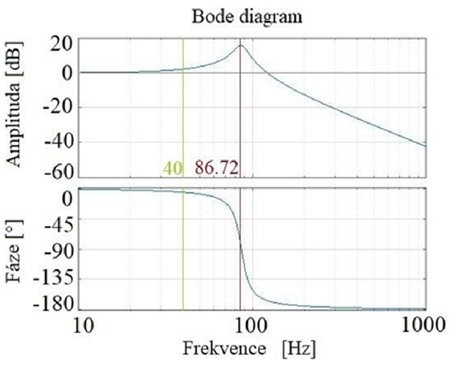
\includegraphics[width=1\textwidth]{pictures/freq_char_pneu.png}
    \label{fig:pneu_freq_char}
\end{figure}
Při měření srdečních frekvencí např. 120 tepů/min tj. 2 Hz, odpovídá 20. harmonická složka tepu frekvenci $f = 40 \ Hz$. Podle obrázku \ref{fig:pneu_freq_char} srdeční frekvence je amplituda zkreslena o +2 dB a fáze signálu o $^\circ 5$, což jsou akceptovatelné hodnoty.

\section{Vyhodnocení dat z AD převodníků}
Tato sekce se zaměří o popsání charakretistiky 12 bit AD převodníku a 24 bit AD převodníku MCP35651. Měření probíhalo na třech veličinách, vstupní piny byly zkratovány s refereční zemí, na napětí z DPS $3.289 \ V$ a poté pomocí napěťového děliče ze $3.289 \ V$ na $1.630 \ V$.
\subsection{Charakteristika MCP3561}

\subsection{Charakteristika 12 bit AD převodníku STM32}
12 bit AD převodník je součástí MCU STM32F407ZGT6. AD převodník slouží k měření absultní hodnoty tlaku z tlakových sezorů na obou větví pneumatického systému. Vzorkovací frekvence byla zvolena $f_s = 1 \ kHz$.

\begin{figure}[H]
    \caption{Graf počtu hodnot LSB 12 bit AD převodníku při připojení kanálu pro první tlakový sensor k refereční zemi.}
    \label{fig:hist_vacuum1_gnd}
    \begin{tikzpicture}
        \begin{axis}
            [ybar,
                width=\textwidth,
                nodes near coords,
                every node near coord/.append style={xshift=6pt,font=\footnotesize},
                ymin=0,
                xlabel={LSB},
                ylabel={Počet}
            ]
            \addplot [
                hist={bins=22},
                fill=orange!75,
                draw=orange!50!black,
            ]
            table [y index=0] {graphs/vacuum1_gnd.dat};

        \end{axis}
    \end{tikzpicture}
\end{figure}

\begin{figure}[H]
    \caption{Graf počtu hodnot LSB 12 bit AD převodníku při připojení kanálu pro první tlakový sensor k $1.630 \ V$.}
    \label{fig:hist_vacuum1_1_6}
    \begin{tikzpicture}
        \begin{axis}
            [ybar,
                width=\textwidth,
                nodes near coords,
                every node near coord/.append style={xshift=6pt,font=\footnotesize},
                ymin=0,
                xlabel={LSB},
                ylabel={Počet},
                xticklabel style = {font=\tiny}
            ]
            \addplot [
                hist={bins=22},
                fill=orange!75,
                draw=orange!50!black,
            ]
            table [y index=0] {graphs/vacuum1_1_6_v.dat};
        \end{axis}
    \end{tikzpicture}
\end{figure}

\pgfplotstablegetrowsof{graphs/vacuum1_3_3_v.dat}
\begin{figure}[H]
    \caption{Graf počtu hodnot LSB 12 bit AD převodníku při připojení kanálu pro první tlakový sensor k $3.289 \ V$.}
    \label{fig:hist_vacuum1_3_3}
    \begin{tikzpicture}
        \begin{axis}[
                ybar,
                nodes near coords,
                nodes near coords align={vertical},
                every node near coord/.append style={xshift=7pt,font=\footnotesize},
                % every node near coord/.append style={xshift=60pt,yshift=-3pt,anchor=west,font=\footnotesize},
                ymin=0,
                width=\textwidth,
                xlabel={LSB},
                ylabel={Počet},
                % xticklabel style = {font=\tiny},
            ]

            \addplot [
                hist={},
                fill=orange!75,
                draw=orange!50!black,
            ]
            table [y index=0] {graphs/vacuum1_3_3_v.dat};
        \end{axis}
    \end{tikzpicture}
\end{figure}











\begin{figure}[H]
    \caption{Graf počtu hodnot LSB 12 bit AD převodníku při připojení kanálu pro druhý tlakový sensor k refereční zemi.}
    \label{fig:hist_vacuum2_gnd}
    \begin{tikzpicture}
        \begin{axis}[
                ybar,
                nodes near coords,
                every node near coord/.append style={xshift=6pt,font=\footnotesize},
                ymin=0,
                width=\textwidth,
                % title=\texttt{Histogram},
                xlabel={LSB},
                ylabel={Počet}
            ]

            \addplot[
                hist={bins=22},
                fill=orange!75,
                draw=orange!50!black,
            ]
            table [y index=0] {graphs/vacuum2_gnd.dat};
        \end{axis}
    \end{tikzpicture}
\end{figure}

\begin{figure}[H]
    \caption{Graf počtu hodnot LSB 12 bit AD převodníku při připojení kanálu pro druhý tlakový sensor k $1.630 \ V$.}
    \label{fig:hist_vacuum2_1_6}
    \begin{tikzpicture}

        \begin{axis}[
                ybar,
                nodes near coords,
                every node near coord/.append style={xshift=6pt,font=\footnotesize},
                % every node near coord/.append style={xshift=60pt,yshift=-3pt,anchor=west,font=\footnotesize},
                ymin=0,
                width=\textwidth,
                % title=\texttt{Histogram},
                xlabel={LSB},
                ylabel={Počet},
                xticklabel style = {font=\tiny}
            ]

            \addplot [
                hist={bins=20},
                fill=orange!75,
                draw=orange!50!black,
            ]
            table [y index=0] {graphs/vacuum2_1_6_v.dat};
        \end{axis}
    \end{tikzpicture}
\end{figure}
\begin{figure}[H]
    \caption{Graf počtu hodnot LSB 12 bit AD převodníku při připojení kanálu pro druhý tlakový sensor k $3.289 \ V$.}
    \label{fig:hist_vacuum2_3_3}
    \begin{tikzpicture}

        \begin{axis}[
                ybar,
                nodes near coords,
                nodes near coords align={vertical},
                every node near coord/.append style={xshift=7pt,font=\footnotesize},
                % every node near coord/.append style={xshift=60pt,yshift=-3pt,anchor=west,font=\footnotesize},
                ymin=0,
                width=\textwidth,
                % title=\texttt{Histogram},
                xlabel={LSB},
                ylabel={Počet},
                % xticklabel style = {font=\tiny},
            ]

            \addplot [
                hist={},
                fill=orange!75,
                draw=orange!50!black,
            ]
            table [y index=0] {graphs/vacuum2_3_3_v.dat};
        \end{axis}
    \end{tikzpicture}
\end{figure}